%   Results
%   Difficulties, limitations, and future works

\section{Results}

\begin{frame}{Results}

    \begin{figure}[H]
    \centering
    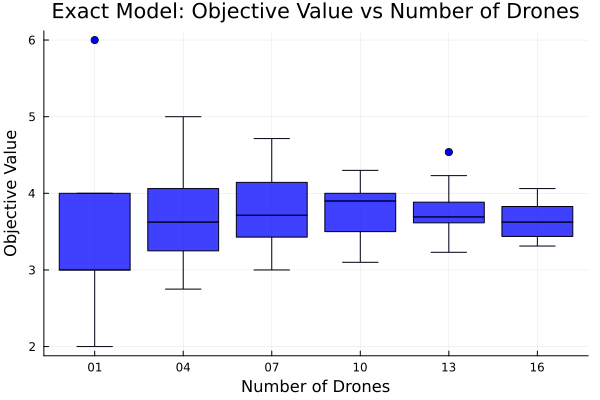
\includegraphics[width=0.57\textwidth]{img/julia_obj_boxplot_vs_drones.png}
    \caption{Exact Model Objective. Source: The authors.}
    \label{fig:exact_model_obj}
\end{figure}

\end{frame}

\begin{frame}{Results}

    \begin{figure}[H]
    \centering
    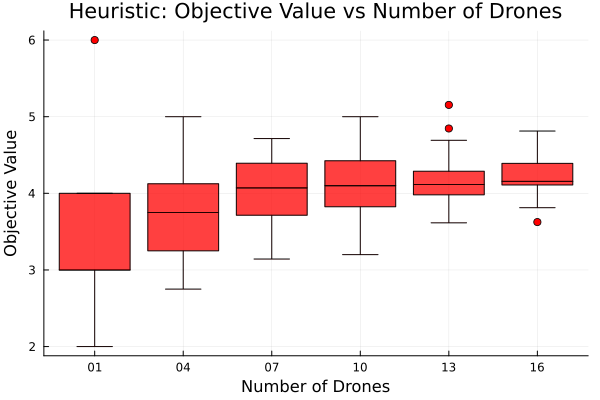
\includegraphics[width=0.57\textwidth]{img/cpp_obj_boxplot_vs_drones.png}
    \caption{Heuristic Objective. Source: The authors.}
    \label{fig:exact_model_obj}
\end{figure}

\end{frame}

\begin{frame}{Results}

\begin{figure}[H]
    \centering
    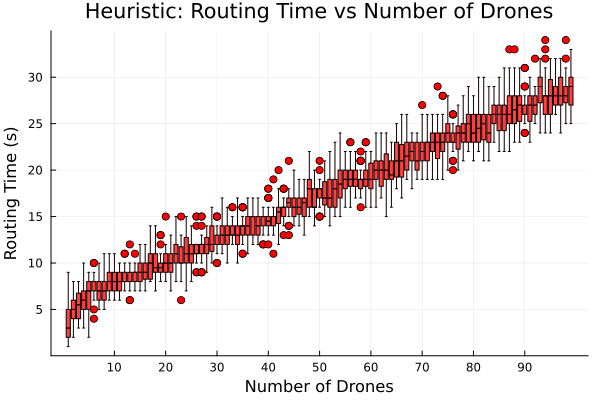
\includegraphics[width=0.57\textwidth]{img/cpp_routing_time_boxplot_vs_drones.png}
    \caption{Heuristic Routing Time ($T$) corresponding to Figure \ref{fig:heuristic_normalized_dist}. Source: The authors.}
    \label{fig:heuristic_normalized_routing_time}
\end{figure}


\end{frame}

% \begin{frame}{Results}



% \begin{figure}
%     \centering
%     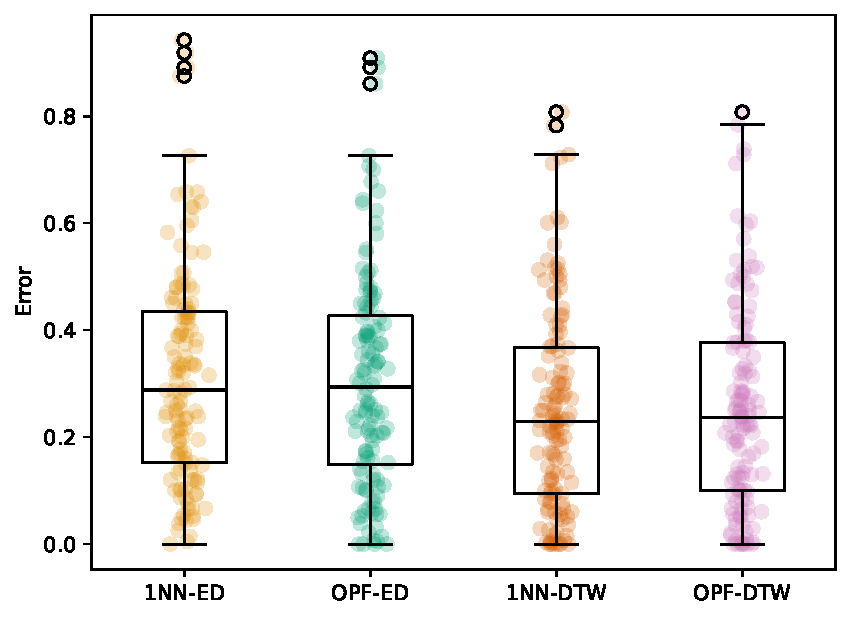
\includegraphics[width=0.5\linewidth]{img/boxplot.pdf}
%     \caption{Boxplot of classification errors for each classifier algorithm. Source: The authors.}
% \end{figure}

% \end{frame}

% \begin{frame}{Results}

% \begin{table}[!htbp]

% \begin{tabular}{ccccc}
% Algorithm & Mean &  Stdev & Wins/Draws/Losses & Wins/Draws/Losses \\
% & ($\mu$) & ($\sigma$) & against 1NN-ED & against 1NN-DTW\\
% \midrule
% OPF-ED & 0.30 & 0.20 & 37/25/66 & 35/7/86\\
% OPF-DTW & 0.25 & 0.19 & 85/7/36 & 14/36/78\\
% 1NN-ED & 0.31 & 0.20 & 0/128/0 & 38/4/86\\
% 1NN-DTW & 0.25 & 0.19 & 86/4/38 & 0/128/0\\
% \end{tabular}%
	
% 	\caption{Mean and standard variation of classification errors for each algorithm, and also the number of times they achieved a better, equal, and worst error than 1NN-ED and 1NN-DTW. Source: The authors.}%
% 	\label{tab:describe_errors} 
% \end{table}

% \end{frame}


